% !TeX root = ../../progress-sem1.tex
% 3.x สถาปัตยกรรมโดยภาพรวมของระบบ
\section{สถาปัตยกรรมโดยภาพรวมของระบบ}
\begin{figure}[H]
  \centering
  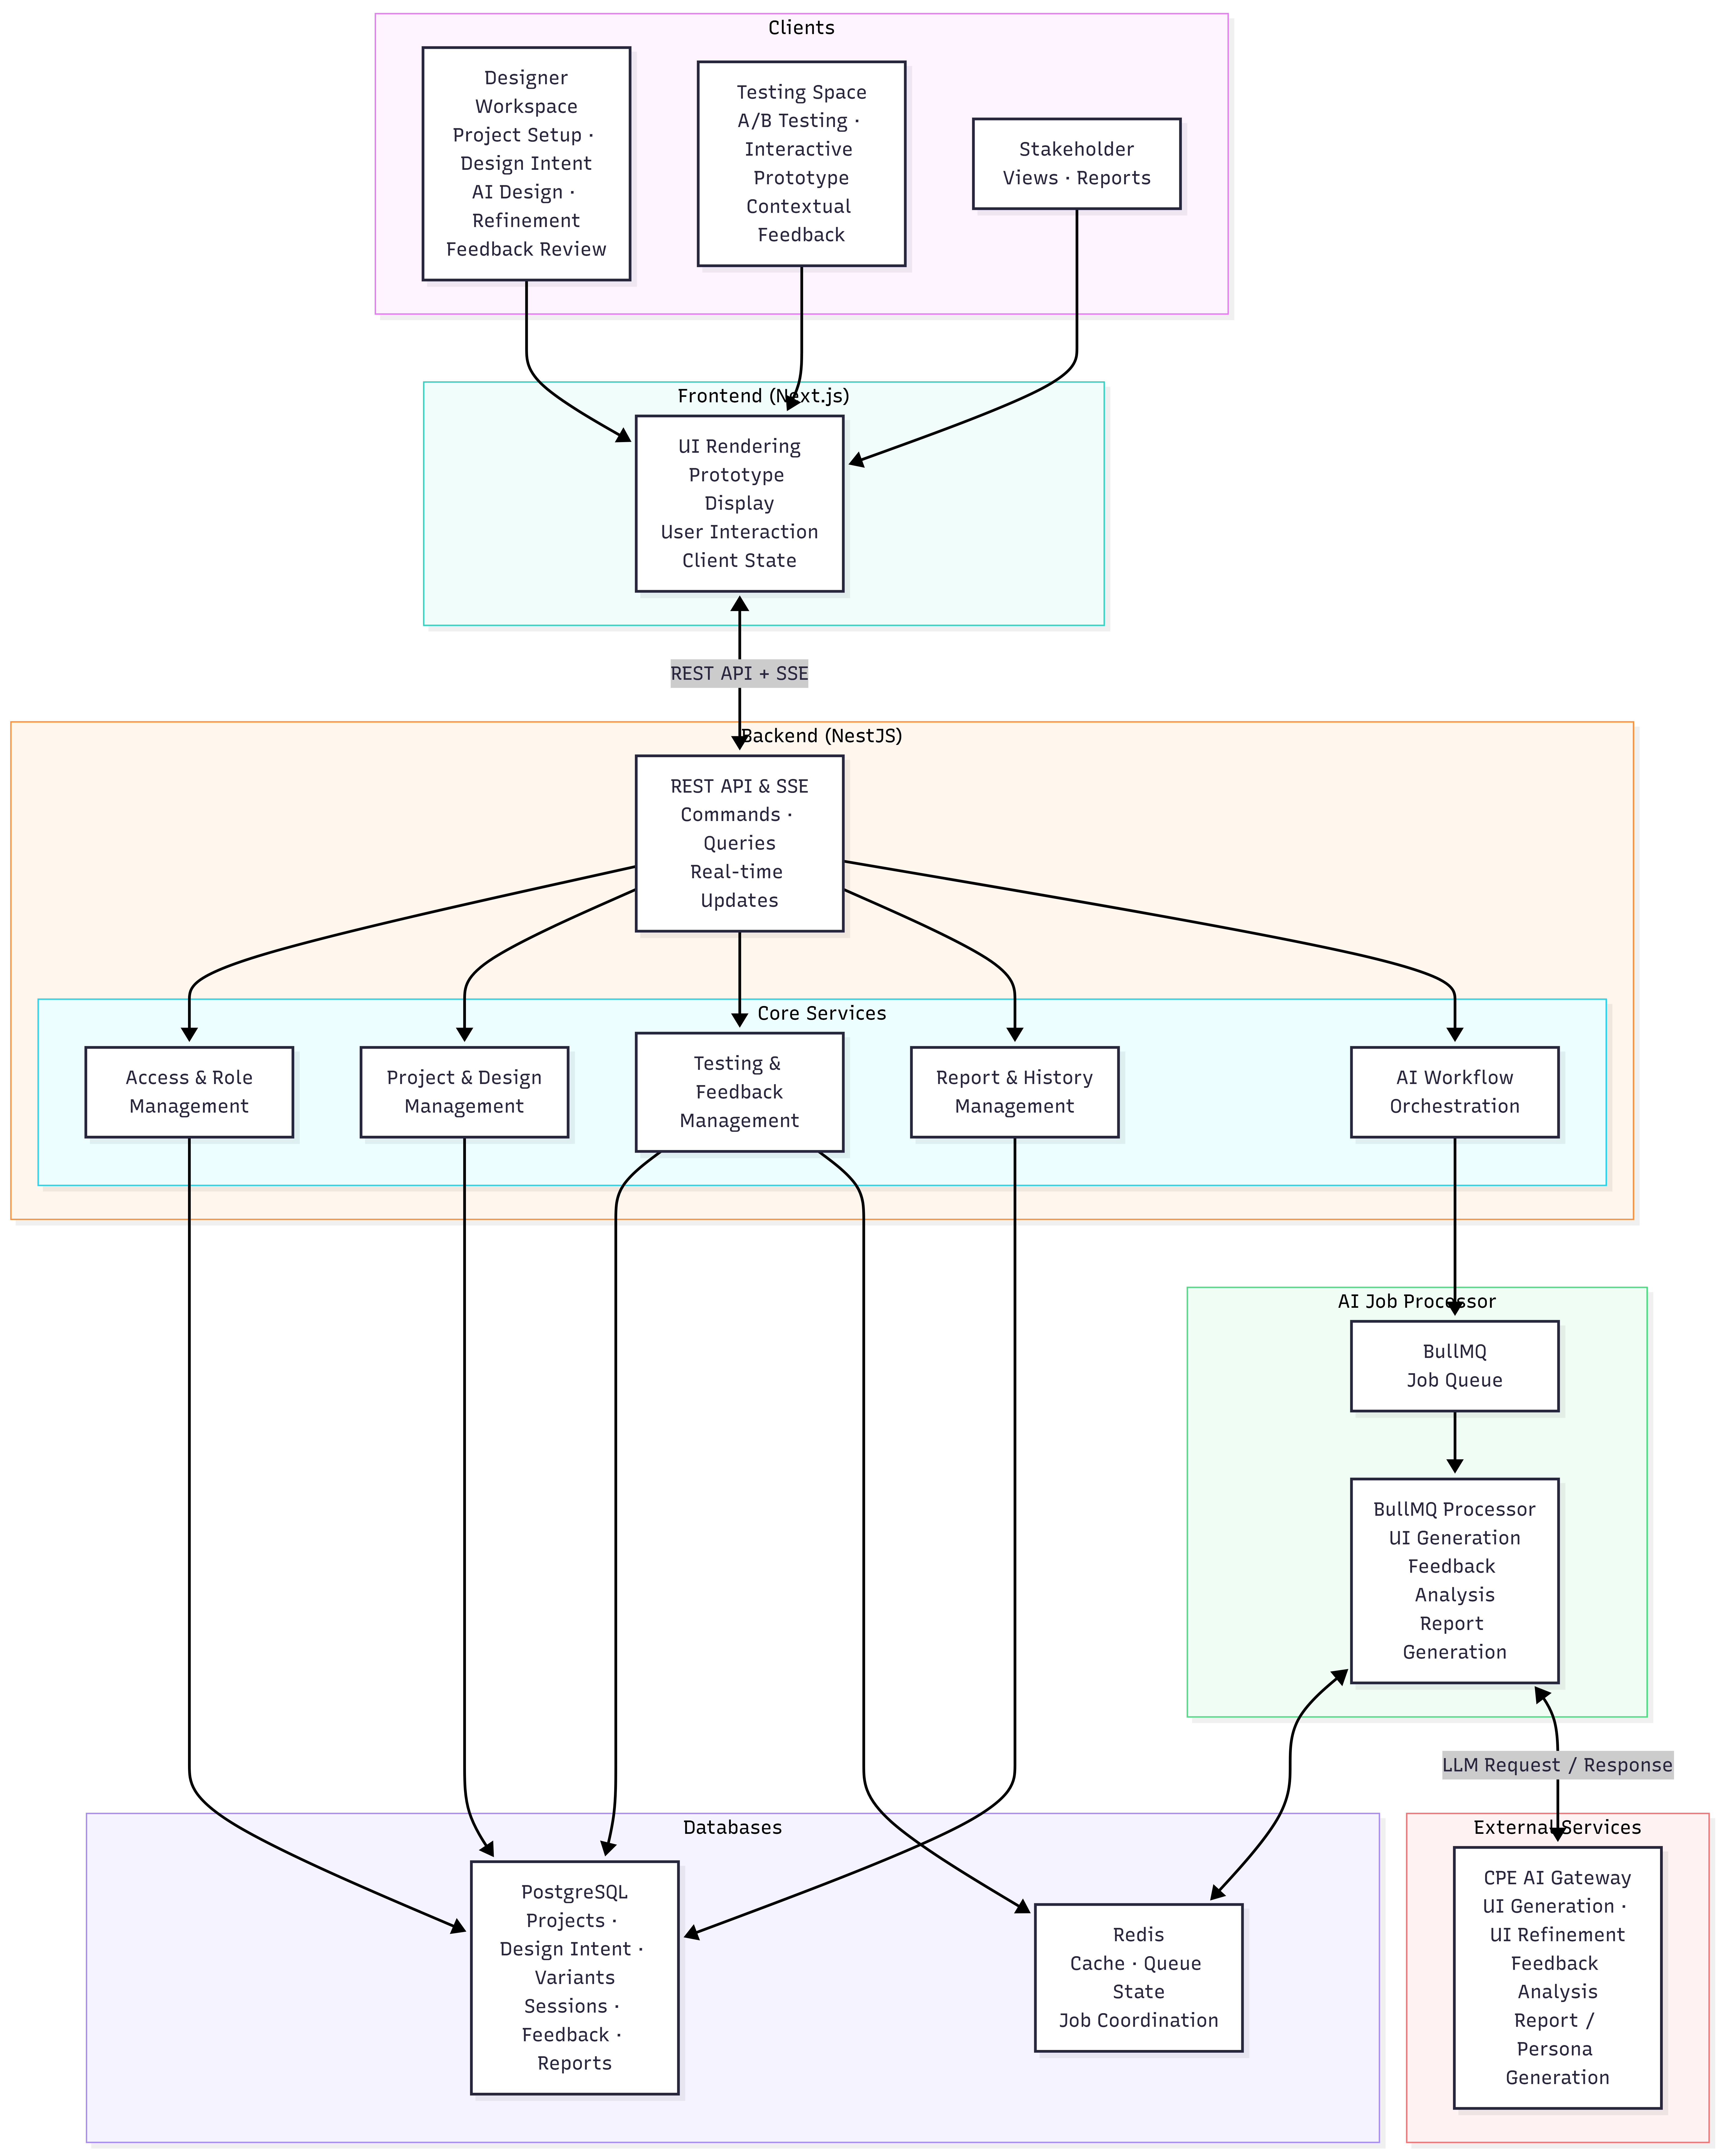
\includegraphics[
    width=0.8\linewidth,
    height=\textheight,
    keepaspectratio
  ]{figures/ch3-methodology/sys-arch3.png}
  \caption{System architecture}
  \label{fig:tech-stack-system-architecture}
  \thaijustify{ภาพแสดงสถาปัตยกรรมระบบโดยแบ่งออกเป็น Client, Frontend, Backend, AI Job Processor, Database และ External Services โดย Frontend พัฒนาด้วย Next.js และสื่อสารกับ Backend ผ่าน REST API และ SSE (Server-Sent Events) ซึ่งช่วยให้ Server สามารถส่งข้อมูลและการอัปเดตแบบ Real-time ไปยัง Client ได้โดยไม่ต้องส่ง Request ใหม่ ขณะที่ Backend ซึ่งพัฒนาด้วย NestJS ทำหน้าที่จัดการสิทธิ์ ข้อมูลโครงการ การทดสอบ Feedback รายงาน และกระบวนการ AI โดยงานที่ต้องใช้เวลาประมวลผลจะถูกส่งผ่าน BullMQ ไปยัง AI Job Processor และเชื่อมต่อกับ CPE AI Gateway สำหรับการประมวลผลด้วย AI}
\end{figure}

% !TeX root = ../../progress-sem1.tex
% Section 3.4 (subsections): one subsection per layer of the system architecture,
% matching "สถาปัตยกรรมโดยภาพรวมของระบบ" in Progress_Sem1_THAI_Example1.pdf.
% Input from chapters/03-methodology.tex, after the architecture figure.

\subsection{Client Side (ส่วนผู้ใช้งาน)}
\thaijustify{
  ผู้ใช้ทุกบทบาทเข้าใช้งานผ่านเว็บเบราว์เซอร์ นักออกแบบ (Designer) ใช้หน้าจอหลักของแพลตฟอร์มตั้งแต่การสร้างโปรเจกต์จนถึงการปรับแก้ UI ผู้เข้าร่วมทดสอบ (Usability Tester) เข้าร่วมเซสชันผ่านลิงก์เชิญโดยไม่ต้องสมัครสมาชิก ส่วน Client, Developer และ Project Manager ใช้มุมมองสำหรับติดตามสถานะ รับมอบงาน และดูรายงาน
}

\subsection{Frontend Layer}
\thaijustify{
  Frontend พัฒนาด้วย Next.js แบบ App Router แบ่ง route ออกเป็นกลุ่ม \texttt{(auth)} สำหรับการเข้าสู่ระบบ \texttt{(dashboard)} สำหรับ workspace และโปรเจกต์ และ \texttt{(legal)} สำหรับนโยบายความเป็นส่วนตัวและข้อกำหนดการใช้งาน หน้าจอสื่อสารกับ backend ผ่าน REST API และรับความคืบหน้าของงาน AI ผ่าน SSE หน้าตัวอย่าง UI ที่ AI สร้างแสดงใน iframe ที่ไม่อนุญาตให้รันสคริปต์ เพื่อป้องกันโค้ดที่ไม่ปลอดภัยจากผลลัพธ์ของโมเดล
}

\subsection{Backend API Layer}
\thaijustify{
  Backend พัฒนาด้วย NestJS แบบ monolith แบ่งเป็น module ตามโดเมน ได้แก่ \texttt{auth}, \texttt{access}, \texttt{users}, \texttt{workspaces}, \texttt{projects}, \texttt{design}, \texttt{rounds}, \texttt{generation}, \texttt{ai}, \texttt{testing}, \texttt{iteration}, \texttt{stakeholders}, \texttt{audit} และ \texttt{health} ทุก request ผ่านการตรวจ token การตรวจสิทธิ์ตาม permission การจำกัดอัตราการเรียก (rate limit) และ security header ก่อนถึง module ปลายทาง
}

\subsection{AI Job Processor Layer}
\thaijustify{
  งานที่ใช้เวลานานถูกส่งเข้าคิวของ BullMQ บน Redis แทนการประมวลผลใน request โดยตรง โดยแบ่งเป็นสองคิว ได้แก่ คิว design-generation สำหรับการสร้าง UI variant และการสังเคราะห์ persona และคิว ai-task สำหรับการร่าง user story และการวิเคราะห์ข้อเสนอแนะ worker ดึงงานจากคิว เรียกโมเดลผ่าน CPE AI Gateway ซึ่งมี API แบบเดียวกับ OpenAI และส่งความคืบหน้ากลับไปยังหน้าจอผ่าน SSE ผู้ใช้จึงปิดหน้าจอแล้วกลับมาติดตามงานเดิมต่อได้ รายละเอียดอยู่ในหัวข้อ~\ref{sec:ai-pipeline}
}

\subsection{Data \& External Services Layer}
\thaijustify{
  PostgreSQL จัดเก็บข้อมูลทั้งหมดของระบบผ่าน Prisma (หัวข้อ~\ref{sec:er-diagram}) Redis ทำหน้าที่ทั้งคิวงานและ cache ของ response บริการภายนอกที่ใช้ ได้แก่ Google OAuth 2.0 สำหรับการเข้าสู่ระบบ และ CPE AI Gateway ของภาควิชาซึ่งเข้าถึงได้ผ่าน VPN ของมหาวิทยาลัยเท่านั้น
}


\subsection{เทคโนโลยีที่ใช้ในแต่ละส่วน}
\thaijustify{
  ซอร์สโค้ดทั้งหมดจัดเก็บใน repository เดียวแบบ monorepo จัดการด้วย Turborepo และ pnpm แบ่งเป็นสองแอปพลิเคชัน คือ frontend และ backend เทคโนโลยีที่ใช้ในแต่ละส่วนแสดงในตารางที่~\ref{tab:tech-stack}
}
\begin{table}[H]
  \centering
  \caption{เทคโนโลยีที่ใช้ในแต่ละส่วนของระบบ}
  \label{tab:tech-stack}
  \small
  \begin{tabularx}{\linewidth}{|>{\RaggedRight\arraybackslash}p{0.2\linewidth}|>{\RaggedRight\arraybackslash}p{0.3\linewidth}|>{\RaggedRight\arraybackslash}X|}
    \hline
    \textbf{ส่วนของระบบ} & \textbf{เทคโนโลยี} & \textbf{หน้าที่} \\ \hline
    Frontend & Next.js 16, React 19, TypeScript & หน้าจอของผู้ใช้ทุกบทบาท \\ \hline
    UI library & shadcn/ui (Radix UI), Tailwind CSS, Hugeicons & component และไอคอนตาม design system ของแพลตฟอร์ม \\ \hline
    Backend & NestJS 11, TypeScript & REST API, การยืนยันตัวตน, การควบคุมสิทธิ์ และงาน AI \\ \hline
    ฐานข้อมูล & PostgreSQL 17, Prisma 7 & จัดเก็บข้อมูลทั้งหมด และจัดการ migration ของ schema \\ \hline
    Cache และคิวงาน & Redis 7, BullMQ & cache ของ response และคิวงานที่ใช้เวลานาน เช่น การสร้าง UI \\ \hline
    การสื่อสารแบบ real-time & Server-Sent Events (SSE) & ส่งความคืบหน้าและความคิดของโมเดลระหว่างประมวลผลไปยังหน้าจอ \\ \hline
    การยืนยันตัวตน & Passport (Google OAuth 2.0), JWT & เข้าสู่ระบบและออก access token กับ refresh token \\ \hline
    บริการ AI & CPE AI Gateway (API แบบเดียวกับ OpenAI) & muse-glimmer-30b สร้าง UI และ qwen3.8-27b วิเคราะห์ข้อเสนอแนะ ร่าง user story, prompt และ persona \\ \hline
    เอกสาร API & Swagger (OpenAPI) & เอกสารและเครื่องมือทดลองเรียก API \\ \hline
    การทดสอบ & Jest & unit test และ end-to-end test ของ backend \\ \hline
    CI & GitHub Actions & ตรวจชื่อ pull request, lint และ build ทุก pull request \\ \hline
  \end{tabularx}
\end{table}
